%% IFB Assignment Latex Template Version 1.0, a fork of :
%% 	RiSE Latex Template - version 0.5
%%
%% IFB Assignment latex template for thesis and dissertations
%% https://github.com/IFBmodels/assignment
%%
%% (c) 2017 Rafael de Campos Passos (rcpassos@ieee.org)
%%
%% This document was initially based on RiSE Latex template, from Yguaratã
%% Cerqueira Cavalcanti
%%
%% GENERAL INSTRUCTIONS
%%
%% We strongly recommend you to compile your documents using pdflatex command.
%% It is also recommend use the texlipse plugin for Eclipse to edit your documents.
%%
%% Options for \documentclass command:
%%         * Idiom
%%           pt   - Portguese (default)
%%           en   - English
%%
%%         * Text type
%%           bsc  - B.Sc. Thesis
%%           msc  - M.Sc. Thesis (default)
%%           qual - PHD qualification (not tested yet)
%%           prop - PHD proposal (not tested yet)
%%           phd  - PHD thesis
%%
%%         * Media
%%           scr  - to eletronic version (PDF) / see the users guide
%%
%%         * Pagination
%%           oneside - unique face press
%%           twoside - two faces press
%%
%%		   * Line spacing
%%           singlespacing  - the same as using \linespread{1}
%%           onehalfspacing - the same as using \linespread{1.3}
%%           doublespacing  - the same as using \linespread{1.6}
%%
%% Reference commands. Use the following commands to make references in your
%% text:
%%          \figref  -- for Figure reference
%%          \tabref  -- for Table reference
%%          \eqnref  -- for equation reference
%%          \chapref -- for chapter reference
%%          \secref  -- for section reference
%%          \appref  -- for appendix reference
%%          \axiref  -- for axiom reference
%%          \conjref -- for conjecture reference
%%          \defref  -- for definition reference
%%          \lemref  -- for lemma reference
%%          \theoref -- for theorem reference
%%          \corref  -- for corollary reference
%%          \propref -- for proprosition reference
%%          \pgref   -- for page reference
%%
%%          Example: See \chapref{chap:introduction}. It will produce
%%                   'See Chapter 1', in case of English language.
%%
%% Citation commands:
%%          \citet (from natbib) -- To cite a reference as part of the narrative
%%          \citep (from natbib) -- To cite a reference between parenthesis
%%          citationblock environment -- To produce direct citation blocks according to the ABNT

\documentclass[pt,oneside,onehalfspacing,acd]{ifbclass/ifbclass}

\usepackage{colortbl}
\usepackage{color}
\usepackage[table]{xcolor}
\usepackage{microtype}
\usepackage{bibentry}
\usepackage{subfigure}
\usepackage{titlesec}
\usepackage{multirow}
\usepackage{rotating}
\usepackage{booktabs}
\usepackage{pdfpages}
\usepackage{caption}
\usepackage{lipsum}
\usepackage{sectsty}
\usepackage{pgfgantt}
\renewcommand{\thesection}{\arabic{section}}

%% Set the language used in your code in the block above

\captionsetup[table]{position=top,justification=centering,width=.85\textwidth,labelfont=bf,font=footnotesize}
\captionsetup[lstlisting]{position=top,justification=centering,width=.85\textwidth,labelfont=bf,font=footnotesize}
\captionsetup[figure]{position=bottom,justification=centering,width=.85\textwidth,labelfont=bf,font=footnotesize}

%% Chapter and (Sub)Section fonts must be same size as text (12)
\sectionfont{\fontsize{12}{15}\selectfont}
\subsectionfont{\fontsize{12}{15}\selectfont}
\subsubsectionfont{\fontsize{12}{15}\selectfont}

%% Change the following pdf author attribute name to your name.
\usepackage[linkcolor=black,
            citecolor=black,
            urlcolor=black,
            colorlinks,
            pdfpagelabels,
            pdftitle={Rise Thesis Template (ABNT)},
            pdfauthor={Rise Thesis Template (ABNT)},
            breaklinks=true]{hyperref}

\address{BRASÍLIA}

\universitypt{Instituto Federal de Brasília}
\universityen{Federal Institute of Brasilia}

\campus{Campus Taguatinga}


%% IF in Academic Assignment Mode (ACD), Define a module:
\module{Processamento de Imagnes}

\programpt{Bacharelado em Ciência da Computação}
\programen{Bachelors in Computer Science}

\majorfieldpt{Ciência da Computação}
\majorfielden{Computer Science}

\title{Título do Trbalho }

\date{2017}

\author{Nome completo do Autor}
\adviser{Nome completo do Orientador}
\coadviser{Nome dompleto do co-orientador }

% Macros (defines your own macros here, if needed)
\def\x{\checkmark}
%\let\lstlistoflistings\origlstoflistings
\begin{document}

\frontmatter

\frontpage

%% IF Document in English, uncoment the Abstract:
%\abstract
%{\parindent0pt
%	Este modelo contém pedaços que podem ser utilizados para formar um trabalho acadêmico pedido por algum módulo ( componente curricular) do curso de Ciência da Computação.

\begin{keywords}
Software Engineering, Software Maintenance and Evolution, Change Request
Management, Automatic Change Request Assignment
\end{keywords}

%% IF Document in Portuguese, uncoment the "Resumo":
\resumo
{\parindent0pt
	Este modelo contém pedaços que podem ser utilizados para formar um trabalho acadêmico pedido por algum módulo ( componente curricular) do curso de Ciência da Computação.

\begin{keywords}
Software Engineering, Software Maintenance and Evolution, Change Request
Management, Automatic Change Request Assignment
\end{keywords}
}
% Summary (tables of contents)
\tableofcontents

\mainmatter


\section{Implementação de Algoritmo}

O algoritmo de determinação de direção pode ser visto no bloco de Algoritmo \ref{code:dir}.
\begin{code}[language=Python,caption=Direction Algorithm,label=code:dir]
import math

def determinant(v1x,v1y,v2x,v2y,v3x,v3y):
    return (v1x * (v2y * 1 - v3y * 1)
           -v2x * (v1y * 1 - v3y * 1)
           +v3x * (v1y * 1 - v2y * 1))

def area(ax,ay,bx,by,cx,cy):
        return ((ax - cx)*(by - cy) - (ay - cy)*(bx - cx))/2

n = int(input())
for i in range(n):
        v1x, v1y, v2x, v2y, v3x, v3y = input().split(' ')
        if dete(v1x,v1y,v2x,v2y,v3x,v3y) is 0:
                print("Indeterminado" )
        else:
                if area(v1x,v1y,v2x,v2y,v3x,v3y) > 0:
                        print("Anti-horario" )
                else:
                        print("Horario" )

\end{code}

\section{Matemática}
Exemplo de bloco Lógico
\subsection{Representações}
Funções Booleanas podem ser representadas de fórma Algébrica e de forma gráfica.\\
Nas funções Booleanas, o operador $\land$ é representado por $ \times $ e podendo ser omitido entre dois termos como na álgebra padrão; e o operador $\lor$ é representado pelo operador $+$ .
\subsubsection{Representação Algébrica}
$\forall$ $x, y$ e $z$ pertencentes ao conjunto de valores $ \cal {B}$,\\
\[f(x)=\neg x\]
\[f(x,y)=\neg x y\]
\[f(x,y,z)=\neg xy+z\]
\[f(x,y,z)=xyz+\neg x \neg y \neg z\]

são fórmulas válidas na representação algébrica de fórmulas booleanas.

\section{Imagem}
Em uma dada arquitetura que utilize 10 Volts como valor padrão, qualquer valor acima de uma voltagem média também definida pela arquitetura representam o valor binário 1 (um), e abaixo representam o valor 0 (zero). Isto pode ser visto na Figura \ref{fig:voltage}

\begin{figure}[h]
    \centering
    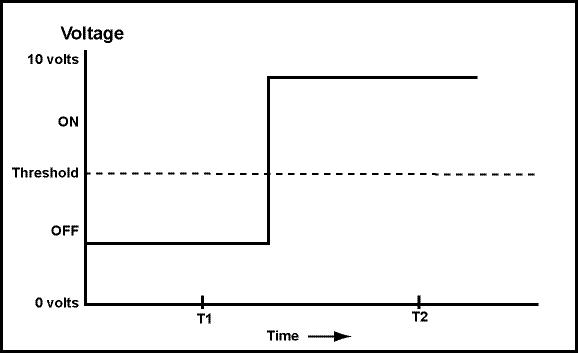
\includegraphics[width=0.85\textwidth]{images/voltage}
    \caption{Gráfico de Sinal digital \cite{centralconnecticutstateuniversity2015}}
    \label{fig:voltage}
\end{figure}

\newpage
\section{Tabela}

As metas do trabalho podem ser vistas na Tabela \ref{table:met}
\begin{table}[h]
\centering
\begin{tabular}{|l | l|}
\hline
\textbf{Objetivos Específicos} & \textbf{Metas}\\
\hline
Versionamento Colaborativo & Trabalho em equipe com colaboração \\
\hline
Centralização de repositórios & Segurança\\
\hline
Melhor escrita & Melhores trabalhos.\\
\hline
Facilitar o Trabalho & Melhores adaptações.\\
\hline
Utilizar \LaTeX & Padronização mais simples.\\
\hline
Padronização com \LaTeX & Fácil reutilização de modelos\\
\hline
Organização e Acompanhamento  & Melhor desempenho acadêmico\\
\hline
Metodologias ágeis & Maiores possibilidades de projetos\\
\hline
Fazer um bom trabalho & Obter uma boa nota\\
\hline
Coluna 1 ( seguida de e-comercial) & coluna 2\\
\hline
\end{tabular}
\caption{Tabela de Objetivos e Metas}
\label{table:met}
\end{table}

\section{Cronograma}
Para desenham um cronograma de acordo com o ciagrama de Gantt, siga como mostrado neste modelo, ou busque pela bibilioteca \textit{pgfgantt}.
\par
Projeto deve ser executado de acordo com o Cronograma na Figura: \ref{fig:gantt}.

%%%Código de geração de gráfico
\begin{figure}[h!]
\begin{center}
\definecolor{barblue}{RGB}{153,204,254}
\definecolor{groupblue}{RGB}{51,102,254}
\definecolor{linkred}{RGB}{165,0,33}
\renewcommand\sfdefault{phv}
\renewcommand\mddefault{mc}
\renewcommand\bfdefault{bc}
\setganttlinklabel{s-s}{}
\setganttlinklabel{f-s}{}
\setganttlinklabel{f-f}{}
\sffamily
\begin{ganttchart}[
    canvas/.append style={fill=none, draw=black!5, line width=.75pt},
hgrid style/.style={draw=black!5, line width=.75pt},
vgrid={*1{draw=black!5, line width=.75pt}},
  today rule/.style={
    draw=black!64,
    dash pattern=on 3.5pt off 4.5pt,
    line width=1.5pt
  },
  today label font=\small\bfseries,
  title/.style={draw=none, fill=none},
  title label font=\bfseries\footnotesize,
  title label node/.append style={below=7pt},
  include title in canvas=false,
  bar label font=\mdseries\small\color{black!70},
  bar label node/.append style={left=2cm},
  bar/.append style={draw=none, fill=black!63},
  bar incomplete/.append style={fill=barblue},
  bar progress label font=\mdseries\footnotesize\color{black!70},
  group incomplete/.append style={fill=groupblue},
  group left shift=0,
  group right shift=0,
  group height=.5,
  group peaks tip position=0,
  group label node/.append style={left=.6cm},
  group progress label font=\bfseries\small,
  link/.style={-latex, line width=1.5pt, linkred},
  link label font=\scriptsize\bfseries,
  link label node/.append style={below left=-2pt and 0pt}
]{1}{12}
%%%
%%% Código de customização do gráfico
\gantttitle[
  title label node/.append style={below left=7pt and -3pt}
]{Mês:\quad1}{1}
\gantttitlelist{2,...,13}{1} \\
\ganttgroup[]{Bolsista 1}{1}{12} \\
\ganttbar[name=refbibi1]{\textbf{Revisão Bibliográfica}}{1}{1} \\
\ganttbar[
  name=projd
]{\textbf{Projeto e Execução}}{2}{3} \\
\ganttbar[
  name=clust
]{\textbf{Criação do Cluster}}{4}{5} \\
\ganttbar[
  name=cloud
]{\textbf{Implementação e testes do OpenStack}}{6}{8} \\
\ganttbar[
  name=vpndns
]{\textbf{Configuração do VPN e DNS}}{9}{11} \\
\ganttbar[name=relat]{\textbf{Relatório Final}}{12}{12}

%%%% Desenho das linhas entre as barras
\ganttlink[link type=f-s]{refbibi1}{projd}
\ganttlink[link type=f-s]{projd}{clust}
\ganttlink[link type=f-s]{clust}{cloud}
\ganttlink[link type=f-s]{cloud}{vpndns}
\ganttlink[link type=f-s]{vpndns}{relat}

\end{ganttchart}
\end{center}
\caption{Cronograma de atividades}
\label{fig:gantt}
\end{figure}

\section{Citações}
    Para fazer citações, utilize o comando \textit{citep} ou \textit{cite} de forma que o parâmetro Interno seja o campo inicial de uma citação ( seu alias :  @ARTICLE\{Eastwood1993,...   ) da seguinte maneira  citep\{swebok2004\}, que gera o seguinte resultado: \citep{swebok2004}
    \\
    De acordo com Eastwood, ... \citep{Eastwood1993} ...\\
    Como mostrado por ... \citep{CavalcantiEASE2013} ... \\
    Encontrado no trabalho ... \citep{Bugzilla}...\\
    
\section{Loren Ipsum}
\lipsum[1-2]

% References

\begin{references}
  \bibliography{bib/references}
\end{references}

% Appendix
\end{document}
